\documentclass[Para_study.tex]{subfiles}
%\usepackage{amsmath}
%\usepackage{tikz}
%\usetikzlibrary{hobby}
\tikzset{
  load/.style   = {ultra thick,-latex},
  stress/.style = {-latex},
  dim/.style    = {latex-latex},
  axis/.style   = {-latex,black!55},
}

\begin{document}

%\tikzset{
%  load/.style   = {ultra thick,-latex},
%  stress/.style = {-latex},
%  dim/.style    = {latex-latex},
%  axis/.style   = {-latex,black!55},
%}

% Drawing View
%\tikzset{dimetric2/.style={
%  x={(-0.25cm,0.5cm)},
%  y={(-1cm,0cm)},
%  z={(0.25cm,0.5cm)},
%}}


%\begin{tikzpicture}[dimetric2,scale=0.7]
%      \coordinate (O) at (2,-2,-0.5); 
%       \draw[axis] (O) -- ++(0.5,0,0) %node[below right] {$x$};
%       \draw[axis] (O) -- ++(0,0.5,0) node[above left] {$y$};
%       \draw[axis] (O) -- ++(0,0,0.5) %node[above] {$z$};


%\draw[thick] (0,0,0) -- (10,0,0);
%\draw[thick] (0,0,0) -- (0,5,0);
%\draw[thick] (10,5,0) -- (0,5,0);
%\draw[thick] (10,5,0) -- (10,0,0);


\begin{tikzpicture}
 \node[anchor=south west, inner sep = 0](image) at (0,0,0) {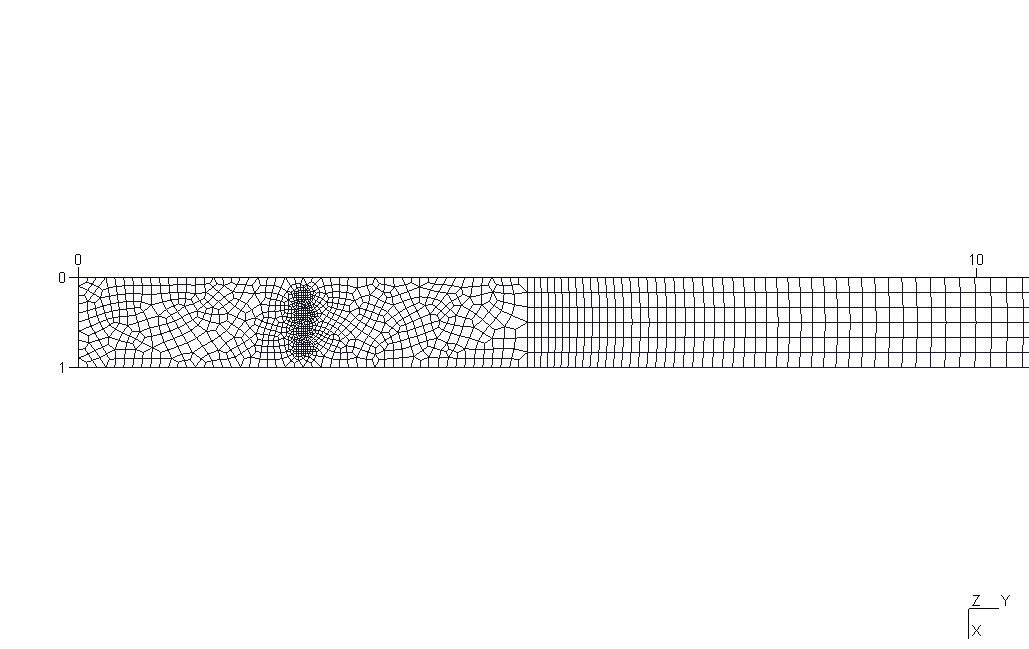
\includegraphics[width=\linewidth,trim={0cm 8cm 0cm 8cm},clip]{Mesh_Dependency/meshes/strip.png}};
 
 \draw[red] (5.55,1.05) -- +(1.1in,-0.6in)node[anchor=west] {Pn2};
 
\draw[red] (5.55,1.505) -- +(1.1in,-0.6in)node[anchor=west] {Pn1};

\draw[red] (5.55,0.6) -- +(1.1in,-0.6in)node[anchor=west] {Pn3};

\draw[green] (0.85,1.505) -- +(0in,-0.38in)node[anchor=north] {$U(t)=sin(wt)$} ;
  
\draw (0.83,1.9) -- (0.83,2.3) ;
\draw (5.55,1.605) -- (5.55,2.3) ;
\draw[dim] (0.83,2.1) -- (5.55,2.1) node [midway,below] {$5m$} ;
\end{tikzpicture}


\end{document}
